\chapter{Introdução}

\label{cap:introducao}

Ao longo dos anos, a computação e suas aplicações se tornaram cada vez mais presentes no nosso cotidiano. Uma
série de fatores contribuiu com a rápida difusão da tecnologia em vários setores, como os ambientes domésticos
e empresariais, com o objetivo de melhorar aspectos de controle, eficiência e gestão.

Embora já na década de 60 casas eletricamente sofisticadas eram construídas, foi durante a primeira metade da
década de 1980 que o termo  ``casa inteligente'' passou a ser utilizado, pois o que determina uma casa
inteligente não é o quão bem é construída ou quão efetiva ela é em relação ao espaço, mas sim as tecnologias
interativas que ela contém. \cite{harper2003}

Para \citeonline{aldrich2003}, uma casa inteligente pode ser definida como uma residência equipada de
tecnologias computacionais que antecipam e respondem às necessidades dos ocupantes, promovendo conforto,
conveniência, segurança e entretenimento através do gerenciamento da tecnologia interna e conexões com o mundo
afora.

Além disso, como a redução de consumo elétrico é um dos principais atrativos em uma casa inteligente, ela
normalmente possui integrações com fontes de energias renováveis, como a solar e a eólica.

O termo domótica origina-se da junção das palavras \textit{domus}, latim para "casa", e robótica, que remete à
automação. Sendo assim, domótica pode ser traduzida como automação residencial, porém, grande parte de seus
conceitos também pode ser aplicada a diversos ambientes como escritórios, indústrias, entre outros.

Segundo \citeonline{riley2012}, domótica é um produto ou serviço que proporciona algum nível de ação ou
mensagem para o ambiente domiciliar, um evento que foi gerado sem a intervenção direta do morador. Um
despertador ou um alarme de incêndio são exemplos disso, porém, esses dispositivos autônomos não
necessariamente possuem um mecanismo de comunicação entre eles, limitando o nível da automação e inteligência
da solução.

Sob uma perspectiva técnica, automação residencial consiste em cinco princípios: dispostivos sob controle, que
são todos os eletrodomésticos e eletrônicos de consumo que estão conectados e controlados pelo mesmo sistema
de automatização; sensores e atuadores, que agem como os olhos e mãos da rede residencial medindo e
controlando o ambiente; dispositivos de controle remoto, como um \textit{smartphone}, que possibilitam a
interação do usuário com a aplicação; controlador, um sistema computacional que coleta informações através dos
sensores e recebe comandos através do dispositivo de controle remoto; e redes de controle, que fornecem a
comunicação entre as tecnologias envolvidas. \cite{kyas2013}

Em relação à rede de controle, essa pode existir em três formatos: sem fio, com fio ou utilizando cabos de
energia elétrica. As três tecnologias têm melhorado significamente em termos de velocidade, confiabilidade e
interoperabilidade através da padronização nos últimos dez anos. \cite{kyas2013}

Contudo, ainda hoje não há um protocolo de comunicação que seja inteiramente adotado, em parte devido ao fato
de requerer que os fabricantes concordem em criar eletrônicos com as mesmas interfaces e protocolos designados
em seus produtos. Porém, as tentativas em padronizar a comunicação na domótica existem desde quase seu início.
Uma das primeiras tentativas foi o X10, que utilizava a rede elétrica existente para transmitir mensagens
através de pulsos codificados, mas devido a diversos problemas, como degradação de sinal e dificuldade para
verificação de pacotes, ele acabou não ganhando muita aceitação. \cite{riley2012}

A expectativa é que todos os dispositivos eletroeletrônicos possuam conexão à internet, conceito que vem sendo
chamado de Internet das Coisas e que prevê o endereçamento único para todos os nós conectados na rede mundial
através da implantação do IPv6. Este último é uma evolução do protocolo de rede IPv4 e surgiu em 1994 com a
intenção de resolver a limitação de espaço de endereço prevista e fornecer funcionalidades adicionais.
\cite{hagen2002}

Entretanto, a adoção do IPv6 de forma unânime ainda não aconteceu mesmo depois de duas décadas desde sua
criação. Além disso, sua utilização completa em domótica levanta a questão quanto à necessidade em conectar
dispositivos simples como sensores e atuadores à \textit{internet}, levando em consideração custo de
implementação e vulnerabilidade. Alternativamente, existe a possibilidade em desenvolver uma rede específica
para esses transdutores, permitindo implementar o monitoramento de um ambiente inteligente de maneira simples
e eficaz.

Essa rede específica, conhecida como rede de sensores [e atuadores], é uma infraestrutura composta por
dispositivos de medição e atuação, de computação e de comunicação que possibilitam instrumentar, observar e
reagir à eventos e fenômenos em um determinado ambiente. \cite{sohraby_minoli_znati2007}

Os quantitativos físicos que podem ser medidos são diversos, como temperatura, umidade, som, luz, radiação,
etc. Como consequência, são várias as possibilidades de aplicação. Algumas das mais comuns são automação
residencial e comercial, monitoramento ambiental e industrial, controle de tráfego, aplicações militares e
assistência médica. A complexidade da rede deve ser proporcial à sua aplicação e vários aspectos devem ser
levados em consideração, como por exemplo o meio de comunicação optado.  \cite{kuorilehto2007}

A utilização de fios para realizar tal tarefa é normalmente descartada devido a diversos fatores como custo,
manutenção, localização e mobilidade. Portanto, uma comunicação sem fio, na maioria dos cenários, é um
requisito inevitável. Com isso, surgiu o termo Rede de Sensores Sem Fio (RSSF), que, apesar do nome,
frequentemente também inclui atuadores.  \cite{karl_willig2005}

A Figura \ref{figura:wsn} ilustra um sistema de domótica utilizando uma rede sem fio para comunicação apenas
com os sensores e atuadores ao invés de uma única rede de controle entre todos os dispotivos.

\begin{figure}[h]
	\centering
	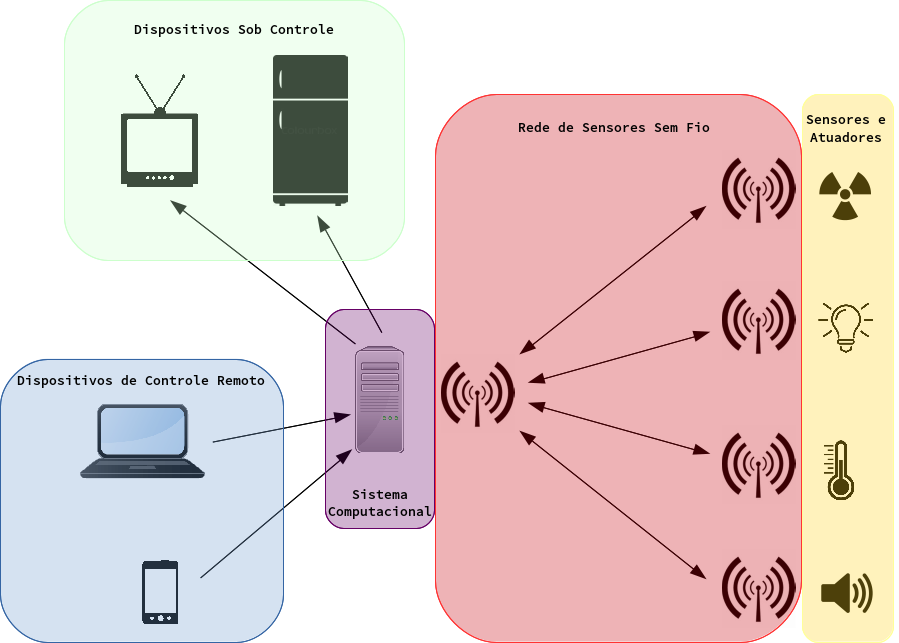
\includegraphics[width=350]{../images/wsn.png}
	\caption{Esboço de uma automação residencial}
	\label{figura:wsn}
\end{figure}

Para este caso é preferível que a implementação da RSSF seja simples, a fim de obter uma solução com baixo
custo e baixo consumo de eletricidade. Sendo assim, é necessário escolher a tecnologia adequada para tal
feito. O protocolo Wi-Fi, por exemplo, foi taxado como muito complexo e com suporte a largura de banda maior
que o necessário; já sistemas infravermelho requerem uma linha de visão, o que nem sempre é possível neste
caso. A tecnologia Bluetooth, por sua vez, aparentou ser promissora no início mas logo foi julgada como cara e
complexa. \cite{sohraby_minoli_znati2007}

Enquanto isso, o uso da comunicação por radiofrequcência tem se tornado cada vez mais abrangente, indo desde
as aplicações tradicionais, como transmissão de sinais de rádio e televisão, para as mais diversas utilidades,
como monitoramento de pacientes em um hospital, \textit{mouses} e teclados sem fio, identificação por
radiofrequência (RFID) e, naturalmente, redes de sensores sem fio. \cite{misra2001}

O padrão IEEE 802.15.4 é uma especificação de comunicação por radiofrequência de baixo alcance projetado para
ter baixa complexidade, baixo custo, baixo consumo de energia e baixa taxa de transmissão de dados. Esse
padrão implementa as camadas física e de controle de acesso ao meio (MAC) e é amplamente utilizado na construção de
RSSFs. Além disso, serve como base para outros protocolos que implementam camadas superiores, como por exemplo
o protocolo ZigBee, que fornece mecanismos para entrada e saída em uma rede, segurança de pacotes, roteamento,
descoberta de caminho, entre outros recursos. \cite{buratti2011}

Outro protocolo que se baseia no padrão IEEE 802.15.4 é o 6LoWPAN(\textit{IPv6 over Low power Wireless
Personal Area Networks}), que possibilita o uso eficiente do IPv6 sobre redes sem fio de baixa taxa e baixo
consumo de energia em dispositivos embarcados simples através de uma camada de adaptação e da otimização dos
protocolos relacionados. \cite{shelby_bormann2009}

Porém, os módulos que utilizam esses protocolos sofisticados possuem um preço relativamente maior em relação
aos módulos com funcionamento mais básico e acabam inflando o custo total da RSSF de acordo com o número de
nós da mesma. Portanto, a fim de se obter uma solução barata é necessário utilizar um transceptor simples e
uma unidade de controle externa de baixo custo para implementar as demais funcionalidades não realizadas pelo
módulo.

Como consequência, ao abrir mão das facilidades que os protocolos de comunicação avançados proporcionam, o
esforço requerido para o desenvolvimento de uma RSSF acaba se tornando maior, sendo necessário definir e
implementar diversos aspectos da mesma.

\section {Objetivo}
Desenvolver uma rede de sensores sem fio, simples e eficáz, para aplicação em automação de residências e
escritórios utilizando tecnologias existentes e visando baixo custo e baixo consumo elétrico.

\section {Organização}
Para o melhor entendimento, essa monografia foi organizada da seguinte forma:

\begin{itemize} \item No Capítulo XXX (\ref{cap:XXX}) são descritos....

\item No Capítulo Conclusão (\ref{cap:conclusao}) são apresentadas de forma suscinta as concluões e trabalhos
futuros relacionados com esse trabalho;

\item Por fim, no Apêndice....  \end{itemize}
